This section gives the explanation of architectural pattern and more detailed implementation of the server side. 

% Architecture MV, , JWT for Auth, Websocket Dispatcher, Resource Listening?

\subsection{Architecture}

\subsubsection{MVC Pattern and Project Structure}
To separate the different layers of model, view and controller, \gls{MVC} pattern is used as the basic pattern of the architecture. In the model layer, all data model related concerns such as data shema definitions, data model validation as well as database operations are defined. And Controllers contain the core domain logics, process the data from model layer, and pass the result to view layer.

Since the templates are rendered on the client side, the view layer is just simply stripped. Therefore, basically the controllers response processed data to client side directly without rendering it to views. Figure \ref{fig:server-file-structure-imp} shows the overview of the server's  file structure which is featured with MVC pattern.

\begin{figure}[!htbp]
\centering
\begin{forest}
  for tree={
    font=\ttfamily,
    grow'=0,
    child anchor=west,
    parent anchor=south,
    anchor=west,
    calign=first,
    edge path={
      \noexpand\path [draw, \forestoption{edge}]
      (!u.south west) +(7.5pt,0) |- node[fill,inner sep=1.25pt] {} (.child anchor)\forestoption{edge label};
    },
    before typesetting nodes={
      if n=1
        {insert before={[,phantom]}}
        {}
    },
    fit=band,
    before computing xy={l=15pt},
  }
[server
  [config/
    [index.js]
    [routes.js]
  ]
  [models/]
  [controllers/]
  [index.js]
  [...]
]
\end{forest}
\caption{Overview of server app's file structure}
\label{fig:server-file-structure-imp}
\end{figure}


\begin{enumerate}
\item 
  \textbf{index.js}: the entry point of the whole server app. It will create a server instance and set up configurations for the server. In addition, a connection from server instance to database will be established. After all configurations are done, the server instance will start listening port and waiting for the requests from client.
\item
  \textbf{config/index.js}: config as well as constants for the server. It persists \textit{apiConfig} for example the common prefix of API URL and version of the API. And config for database including the database URL will be defined here as well. In addition, keys for encryption are also stored in the config file.
\item
  \textbf{config/routes.js}: rules for URL matching. All URL matching rules are defined in this file. Controllers are referenced here and a dispatcher for router will be instantiated. If any request meets the defined rule, the request will be forward to a correlative controller. 
\item
  \textbf{controllers/*}: controllers for processing specific requests.
\item 
  \textbf{models/*}: data model definitions. Files under this directory are organized by different data domain.
\end{enumerate}


\subsubsection{Achitecture of Server}

The figure \ref{fig:server-arch-imp} illustrates an overview of the server's architecture. 

\begin{figure}[!htbp]
  \centering
    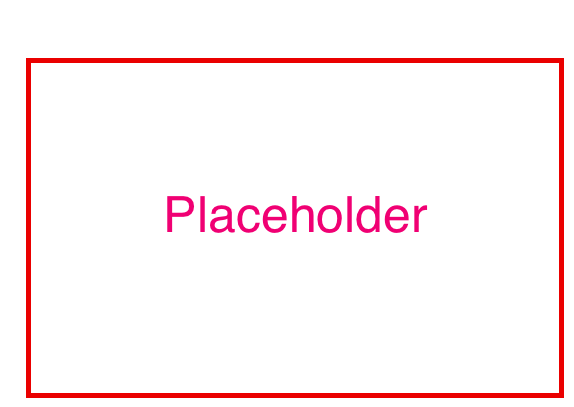
\includegraphics[width=0.6\textwidth]{Figures/placeholder.png}
  \caption{placeholder}
  \label{fig:server-arch-imp}
\end{figure}
% process of request to be handeled. index.js -> create server isntance -> connect to database. routes (different HTTP methods) ->  different controllers (different HTTP methods) -> different models
% layered!!! controller layer, model layer!!!




\subsection{Model Layer Implementation}
In subsection \ref{subsec:storage-structure-imp} an overview of the storage structure has been described. In following subsections, more concrete implementation of data model layer is explained and example codes are represented.

\subsubsection{Data Model Schema}

Not only the fields of each data model are defined, but also data type of each field should also be restricted. Mongoose will check the type of fields within a data model according to the definitions before a record is inserted into the database. 

\begin{lstlisting}[language=JavaScript, caption=Example: user schema definition within Mongoose, label={list:user-schema-def-imp}]
import mongoose from 'mongoose'
const userSchema = mongoose.Schema({
  username: String,
  email: {type: String, lowercase: true, trim: true, unique: true},
  password: {type: String, select: false},
  faculty: {type: String, default: ''},
  tutor: {type: Boolean, default: false},
  admin: {type: Boolean, default: false}
}, {timestamps: true});
\end{lstlisting}

Code list \ref{list:user-schema-def-imp} takes \textit{UserSchema} definition as an example. Fields like \textit{username}, \textit{email}, \textit{password} and \textit{faculty} are defined as \textit{String} type. Fileds like \textit{tutor} and \textit{admin} are using \text{Boolean} type for determining the role of a user. In addition, default value of an field could also be given if record is added without value on this field. And Mongoose also provides a set of configurations for processing the entry inserted. In the example, setting \textit{lowercase} on \textit{email} will transform all characters to lowercase, while setting \textit{trim} will stripped space symbols out of a string. Mongoose will not only validate the type of data model, but also check the uniqueness of the data field in the entire database if \textit{unique} is set to \textit{true}. 

\subsubsection{Methods on Model Layer}
In most cases, various operations are executed to acquire data from the database, modify data and even remove data in the database. Therefore, those data fetching or data processing tasks are implemented in the data model layer, which will also achieve the goal of seperation of concern. A example of \textit{Course} data model is taken in the following code list \ref{list:course-data-method-imp}.

\begin{lstlisting}[language=JavaScript, caption=Example: user schema definition within Mongoose, label={list:course-data-method-imp}]
courseSchema.statics.list = function() {
  return this.find().sort('-createdAt').populate('creator').exec()
}
courseSchema.statics.load = function(_id) {
  return this.findById(_id).populate('creator').exec()
}
courseSchema.method.edit = function(fields) {
  return this.update(fields).exec()
}
courseSchema.method.remove = function() {
  return this.remove().exec()
}
\end{lstlisting}

Other data models like \textit{Question} and \textit{Answer} are quite same as \textit{Course}. Method \textit{list()} is defined for querying all records of a collection under the data domain. In addition, sorting and referencing other model with foreign key will also be done before returning the result. \textit{load()} method is for querying a specific entry. Methods \textit{edit()} and \textit{remove()} means modification or removal of an entry in database.



\subsection{Authentication}
The goal of authentication is confirming the identity of an user and controll the access of resources by checking the privilege of an user. So an authentication system is also designed for security reasons.

\subsubsection{JWT based Authentication}
JSON Web Token (JWT) is an open standard (RFC 7519) that defines a compact and self-contained way for securely transmitting information between parties as a JSON object. This information can be verified and trusted because it is digitally signed. Reference!!!


\begin{figure}[!htbp]
  \centering
    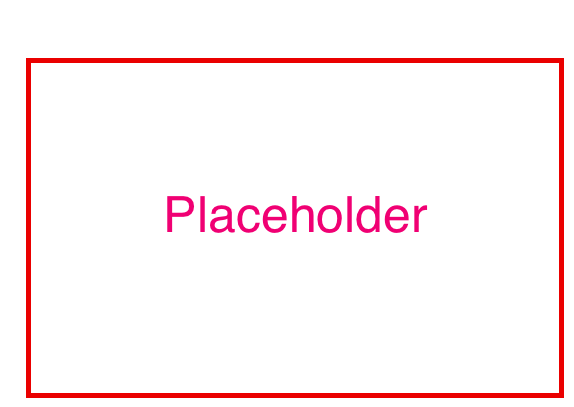
\includegraphics[width=0.6\textwidth]{Figures/placeholder.png}
  \caption{placeholder}
  \label{fig:jwt-process-imp}
\end{figure}
% JWT process! request login -> verification success -> generate token with secret -> write token to cookie -> response. all request after login with token!-> jwt verify!, logout -> remove token!


The basic idea of JWT based Authentication in the server side of Graphicuss is shown in figure \ref{jwp-process-imp}. After that the user sends request to login with its identifier and password and the the authentication is successfully verified, JWT will encode the user information with a secret key to a token.

\begin{lstlisting}[language=JavaScript, caption=JWT encodes user information with secret key, label={list:jwt-encode-imp}]
var token = jwt.sign(userInfo, authConfig.jwtSecret)
response.cookie('token', token);
\end{lstlisting}

After that the authentication is successfully verified and Cookies are written with JWT token, every request started from the client side will be sent with Cookies. All the requests will go through the \textit{authMiddleware} and the tokens inside Cookies from requests will be decoded with the secret key. With the payload of user information which is decoded from the token, server is able to deal with resources for the specific user.

\begin{lstlisting}[language=JavaScript, caption=JWT decodes user information with secret key, label={list:jwt-decode-imp}]
jwt.verify(token, authConfig.jwtSecret, function(err, decoded) {
  var userInfo = decode
})
\end{lstlisting}

\subsubsection{Role Control \& Access Control}
As defined in section \ref{subsec:storage-structure-imp}, each user has two fields called \textit{tutor} and \textit{admin}. An admin has full control of all resources while a tutor  is able to create a course and manage all resources under his course. Same as a normal user without any privileges, he could only maintain resources submitted by himself.

So a \textit{if} statement will be executed before the operations on resources in order to determine the role of the user, or to verify if an user has the access to the specific resource.


% \subsection{Processing of Controller}


\subsection{WebSocket Implementation}
For the implementation of real-time functionality, a library called Socket.io\footnote{http://socket.io/} which a fast and reliable real-time engine is used. 

As described in section \ref{sec:realtime-concept}, at the start of server, an instance of Socket.io will be created for listening for WebSocket requests within specific namespace. Following code list \ref{list:server-websocket-course-listen-imp} shows the main process of listener created for real-time questions under a specific course.

\begin{lstlisting}[language=JavaScript, caption=Server starts listening for requests over WebSocket protocol , label={list:server-websocket-course-listen-imp}]
var courseWS = io.of('/ws/courses/');
var courseSocketMap  = {};
courseWS.on('connection', function(socket){
  socket.on('course-to-listen', function(courseId){
    if(courseSocketMap[courseId]){
      courseSocketMap[courseId].push(socket)
    }
    else{
      courseSocketMap[courseId] = [socket]
    }
  });
});

courseWS.on('disconnection', function(socket){
  Object.keys(courseSocketMap).forEach(function(courseId) {
    var index = courseSocketMap[courseId].indexOf(socket)
    if (index > -1) {
      courseSocketMap[courseId].splice(index, 1);
    }
  });
});
/* --- Listening for Question is the same approach--- */
\end{lstlisting}

After the WebSocket listener is started, it will monitoring the the event called \textit{course-to-listen}. As it is triggered, \textit{courseId} received from client will be mapped to the a list of socket objects which represent the users who are listening to this resource. After the client disconnets from the WebSocket, his socket object will be removed from the listening list. 

\begin{lstlisting}[language=JavaScript, caption=Server starts listening for requests over WebSocket protocol , label={list:server-websocket-course-emit-imp}]
var sockets = courseSocketMap[courseId];
sockets.forEach(function(socket){
  socket.emit('questions-changed', newQuestions);
});
/* --- Listening for Question is the same approach--- */
\end{lstlisting}

If the questions under the specific course are changed, all sockets which could be referenced from \textit{courseSocketMap} by using the \textit{courseId} will emit a event with payload of changed question resources. Those clients who has subscribed this course will be informed and receive the new questions passively. Code list \ref{list:server-websocket-course-emit-imp} demonstrates the process.

The approach of real-time order of answers under a specific question is quite same as the approach mentioned above.